\documentclass[11pt,oneside]{report}

\usepackage[margin=0.9in,headheight=24pt]{geometry}
\usepackage[T1]{fontenc}
\usepackage[utf8]{inputenc}
\usepackage{amsmath,amssymb}
\usepackage{booktabs}
\usepackage{longtable}
\usepackage{array}
\usepackage{xcolor}
\usepackage{tikz}
\usepackage{hyperref}
\usepackage{enumitem}
\usepackage{listings}
\usepackage{titlesec}
\usepackage{fancyhdr}
\usepackage[protrusion=true,expansion=false]{microtype}

\usetikzlibrary{arrows.meta,calc,decorations.pathmorphing,positioning}

\definecolor{Ink}{HTML}{1B2430}
\definecolor{Muted}{HTML}{5B6472}
\definecolor{Accent}{HTML}{0077B6}
\definecolor{AccentTwo}{HTML}{D95F02}
\definecolor{Soft}{HTML}{F5F7FA}
\definecolor{SoftBlue}{HTML}{EAF4FB}
\definecolor{SoftOrange}{HTML}{FFF2E8}

\renewcommand{\familydefault}{\sfdefault}
\setlength{\parindent}{0pt}
\setlength{\parskip}{6pt}
\setlist{itemsep=2pt,topsep=4pt}

\hypersetup{
  colorlinks=true,
  linkcolor=Accent,
  urlcolor=Accent,
  citecolor=Accent
}

\lstdefinestyle{pythonstyle}{
  basicstyle=\ttfamily\small,
  backgroundcolor=\color{Soft},
  columns=fullflexible,
  keepspaces=true,
  breaklines=true,
  frame=leftline,
  framerule=2pt,
  rulecolor=\color{Accent},
  xleftmargin=0.8em,
  framesep=0.6em,
  showstringspaces=false
}
\lstset{style=pythonstyle}

\newcommand{\code}[1]{\texttt{#1}}
\newcommand{\dd}{\,\mathrm{d}}
\newcommand{\ii}{\mathrm{i}}
\newcommand{\scopebox}[2]{%
  \par\smallskip
  \noindent\fcolorbox{#1!55!black}{#1!10}{%
    \begin{minipage}{0.96\linewidth}
    #2
    \end{minipage}}
  \par\smallskip
}
\input{../docs/assets/nmr_spin_dynamics_logo_tikz.tex}

\titleformat{\chapter}[block]
  {\huge\bfseries\color{Ink}}
  {\color{Accent}\thechapter}
  {0.75em}
  {}
\titlespacing*{\chapter}{0pt}{-0.15in}{1.1em}
\titleformat{\section}
  {\Large\bfseries\color{Ink}}
  {\thesection}
  {0.6em}
  {}
\titleformat{\subsection}
  {\large\bfseries\color{Ink}}
  {\thesubsection}
  {0.6em}
  {}

\pagestyle{fancy}
\fancyhf{}
\lhead{\textcolor{Muted}{PythonSpinDynamics}}
\rhead{\textcolor{Muted}{User Manual}}
\cfoot{\textcolor{Muted}{\thepage}}
\renewcommand{\headrulewidth}{0.3pt}
\renewcommand{\headrule}{\hbox to\headwidth{\color{Accent!35}\leaders\hrule height \headrulewidth\hfill}}

\begin{document}
\pagenumbering{gobble}
\begin{titlepage}
\pagecolor{Soft}
\color{Ink}
\vspace*{0.55in}
\begin{center}
\NMRSpinDynamicsLogo[0.85]
\end{center}
\vspace{0.45in}
{\Huge\bfseries PythonSpinDynamics\par}
\vspace{0.25in}
{\Large User Manual\par}
\vspace{0.15in}
{\large Python port of MATLABSpinDynamics\par}
\vspace{0.45in}
{\color{Accent}\rule{0.82\linewidth}{3pt}\par}
\vspace{0.35in}
\begin{minipage}{0.78\linewidth}
\large
Simulation workflows for spin-1/2 nuclear magnetization in possibly
non-uniform and time-varying magnetic fields, with validated
MATLAB-compatible Bloch kernels, Python-native analysis tools, and scoped
scalar-coupled spin-1/2 and pulsed NQR extensions.
\end{minipage}
\vfill
{\large June 2026\par}
\end{titlepage}
\nopagecolor
\clearpage
\pagenumbering{roman}
\tableofcontents
\clearpage
\pagenumbering{arabic}

\chapter{Physical Scope and Assumptions}

The MATLAB-compatible workflow layer in PythonSpinDynamics models a bath of
uncoupled spin-1/2 nuclei evolving in a static, spatially non-uniform, or
time-varying main field \(B_0(\mathbf{r},t)\) and applied RF fields. The
elementary object in that layer is an isochromat: a subensemble of spin-1/2
nuclei that shares an offset, RF sensitivity, relaxation constants, and probe
response.

\scopebox{Accent}{
\textbf{Modeled directly in the core Bloch workflows.} Independent spin-1/2
magnetization vectors; offset distributions from \(B_0(\mathbf{r},t)\); RF
rotations; free precession; phenomenological \(T_1\) and \(T_2\) relaxation;
probe transmit and receive filtering; optional deterministic radiation damping;
optional motion through field maps.
}

\scopebox{Accent}{
\textbf{Scalar-coupling extension.} The \code{spin\_dynamics.coupling}
namespace adds small dense spin-1/2 systems with scalar J couplings, analytic
low-field J-editing models, ideal TANGO-B filter curves, and initial SLIC
simulations. These models are intentionally scoped and are documented in
Chapter~\ref{chap:jcoupling}.
}

\scopebox{Accent}{
\textbf{Pulsed NQR extension.} The \code{spin\_dynamics.nqr} namespace adds
dense single-site quadrupolar spin tools for selective pulsed NQR, including
spin-1 transition metadata, single-crystal and powder orientation averages,
SLSE echo trains, two-frequency population transfer, and weak-B0 perturbations.
These models are documented in Chapter~\ref{chap:nqr}.
}

\scopebox{AccentTwo}{
\textbf{Still outside the package scope.} Dipolar coupling networks, chemical
exchange, arbitrary nonselective multi-quantum pulse sequences, shaped sample
microstructure beyond the supplied field and density maps, microscopic spin
noise, and large sparse coupled-spin simulations. Spin-spin effects enter the
Bloch workflows only indirectly when represented by effective relaxation times
such as \(T_2\) or \(T_2^*\).
}

This scope is deliberate. The main package follows MATLAB's classical
Bloch/isochromat viewpoint, which is appropriate for many pulse, probe,
imaging, and relaxation studies where the spins can be treated as independent
subensembles. The coupled-spin namespace adds targeted quantum spin-1/2 tools
for scalar J-coupling phenomena without turning the full package into a general
quantum spin Hamiltonian framework.

\section{Spin Bath Cartoon}

\begin{center}
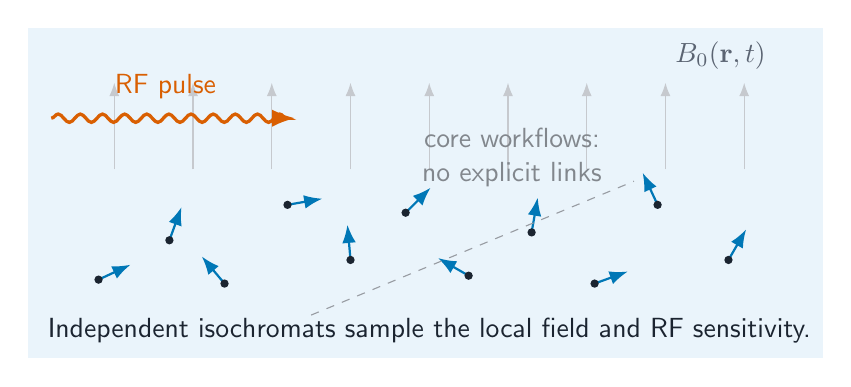
\begin{tikzpicture}[x=1cm,y=1cm,>=Latex]
  \fill[SoftBlue] (-0.4,-0.4) rectangle (9.7,3.8);
  \foreach \x/\y/\a in {
    0.5/0.6/25, 1.4/1.1/70, 2.1/0.55/130, 2.9/1.55/10,
    3.7/0.85/95, 4.4/1.45/45, 5.2/0.65/150, 6.0/1.2/80,
    6.8/0.55/20, 7.6/1.55/115, 8.5/0.85/60}
  {
    \draw[Accent,thick,->] (\x,\y) -- ++(\a:0.45);
    \fill[Ink] (\x,\y) circle (1.5pt);
  }
  \foreach \x in {0.7,1.7,...,8.7}
  {
    \draw[Muted!35,->] (\x,2.0) -- ++(0,1.1);
  }
  \node[Muted] at (8.4,3.45) {$B_0(\mathbf{r},t)$};
  \draw[AccentTwo,very thick,decorate,decoration={snake,amplitude=1.5pt,segment length=8pt},->]
    (-0.1,2.65) -- (3.0,2.65);
  \node[AccentTwo] at (1.35,3.05) {RF pulse};
  \draw[Ink!45,dashed] (3.2,0.15) -- (7.3,1.85);
  \node[Ink!55,align=center] at (5.75,2.15) {core workflows:\\no explicit links};
  \node[align=left,Ink] at (4.7,-0.05) {Independent isochromats sample the local field and RF sensitivity.};
\end{tikzpicture}
\end{center}

\section{Consequences for Users}

\begin{itemize}
  \item Use offset grids, field maps, or moving particles to represent
  spatially varying \(B_0\), transmit \(B_1\), and receive \(B_1\) effects.
  \item Use relaxation constants to represent ensemble dephasing and energy
  exchange that are outside the explicit isochromat model.
  \item Use \code{spin\_dynamics.coupling} when a small spin-1/2 scalar
  J-coupled model is the phenomenon of interest.
  \item Use \code{spin\_dynamics.nqr} when selective pulsed NQR of a small
  quadrupolar site is the phenomenon of interest.
  \item Do not use the package for chemical exchange, large coupled-spin
  networks, or arbitrary nonselective multi-quantum coherence pathways.
\end{itemize}

\chapter{Overview}

PythonSpinDynamics is a Python port of the MATLAB spin-dynamics simulation
package. The MATLAB tree under \code{../MATLABSpinDynamics/SpinDynamicsUpdated/Version\_2/code}
remains the reference for numerical behavior, while this workspace provides a
typed, testable Python API for simulations, validation fixtures, examples, and
new analysis workflows.

The supported surface currently includes ideal, tuned, untuned, and matched
probe CPMG workflows; finite echo trains; FID; phase-encoded imaging; diffusion
CPMG; time-varying-field CPMG; WURST inversion and matched WURST-CPMG;
radiation damping; moving-isochromat motion helpers; received-signal noise;
inverse-Laplace analysis; compact pulse-optimization scaffolds; and small
spin-1/2 scalar-coupling tools for low-field J-editing, TANGO-B filtering, and
SLIC-style spin-lock response; and early pulsed NQR helpers for quadrupolar
sites, powder averaging, SLSE, and two-frequency population transfer.

\section{Package Layout}

\begin{longtable}{p{0.36\linewidth}p{0.56\linewidth}}
\toprule
Path & Purpose \\
\midrule
\code{src/spin\_dynamics/} & Installable Python package. \\
\code{examples/} & CLI examples and plotting scripts. \\
\code{tests/} & Smoke tests, validation tests, and unit tests. \\
\code{validation/fixtures/} & MATLAB/Octave fixture arrays. \\
\code{validation/octave/} & Fixture generation scripts. \\
\code{docs/python\_api/} & Lightweight Markdown API notes. \\
\code{docs/validation\_results.md} & Current validation status and tolerance notes. \\
\code{docs/radiation\_damping.md} & Focused radiation-damping model notes. \\
\bottomrule
\end{longtable}

\chapter{Installation and Test Runs}

\section{Editable Install}

PythonSpinDynamics requires Python 3.10 or newer. The core install depends on
NumPy 1.24 or newer and does not require MATLAB at runtime. MATLAB is only
needed to regenerate the complete MATLAB reference fixture set; Octave can
regenerate the smaller dependency-light fixtures.

From \code{PythonSpinDynamics}, install the package into an active environment:

\begin{lstlisting}[language=bash]
python -m pip install -e .
\end{lstlisting}

Optional extras are provided for development, plotting, benchmarking, and
SciPy-backed optimization:

\begin{lstlisting}[language=bash]
python -m pip install -e ".[dev,opt,plot,bench]"
\end{lstlisting}

The core package depends only on NumPy. The \code{opt} extra enables SciPy-backed
continuous optimizers, non-negative inverse-Laplace solves, and MATLAB
\code{.mat} result import/export helpers. The \code{plot} extra enables the
Matplotlib examples.

\section{Tests}

Use the smoke tier during normal editing:

\begin{lstlisting}[language=bash]
python -m unittest tests.smoke_tests
\end{lstlisting}

Run the full validation suite before committing numerical or workflow changes:

\begin{lstlisting}[language=bash]
python -m unittest discover -s tests
\end{lstlisting}

\chapter{Model Conventions}

\section{Coherence Ordering}

Low-level kernels preserve MATLAB's coherence ordering:
\[
  \mathbf{M} =
  \begin{bmatrix}
    M_0 & M_- & M_+
  \end{bmatrix}^{\mathsf{T}} .
\]
This ordering differs from many Bloch-vector presentations, so new kernels and
validation tests should state the expected ordering explicitly.

\section{Normalized Time}

The core MATLAB routines usually normalize time to the nominal RF amplitude
\( \omega_1 = 1 \). In these units, a 90-degree hard pulse has duration
\[
  t_{90} = \frac{\pi}{2},
\]
and a 180-degree hard pulse has duration
\[
  t_{180} = \pi .
\]
Workflow helpers that expose physical seconds convert into these normalized
units before calling the lower-level kernels.

\section{Pulse Timing Cartoon}

A minimal spin-echo or CPMG building block is a sequence of RF pulses, free
precession windows, and acquisition windows. The package represents these as
ordered intervals with pulse matrices and free-precession delays.

\begin{center}
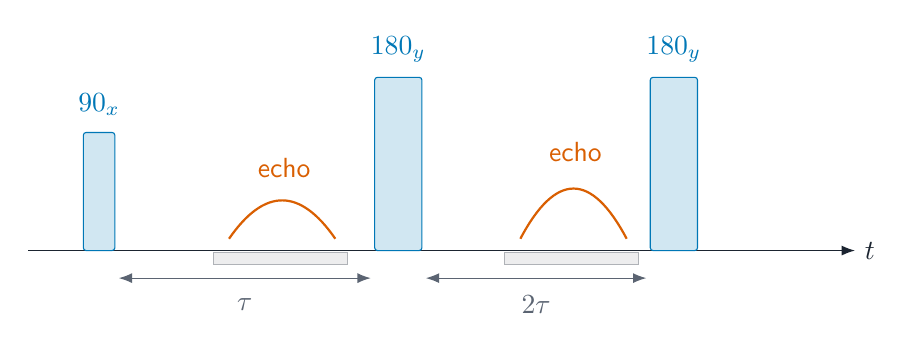
\begin{tikzpicture}[x=1cm,y=1cm,>=Latex]
  \draw[Ink,->] (0,0) -- (10.5,0) node[right] {$t$};
  \draw[Accent,fill=Accent!18,rounded corners=1pt] (0.7,0) rectangle (1.1,1.5);
  \node[Accent] at (0.9,1.85) {$90_x$};
  \draw[Accent,fill=Accent!18,rounded corners=1pt] (4.4,0) rectangle (5.0,2.2);
  \node[Accent] at (4.7,2.55) {$180_y$};
  \draw[Accent,fill=Accent!18,rounded corners=1pt] (7.9,0) rectangle (8.5,2.2);
  \node[Accent] at (8.2,2.55) {$180_y$};
  \draw[Muted,<->] (1.15,-0.35) -- (4.35,-0.35);
  \node[Muted] at (2.75,-0.68) {$\tau$};
  \draw[Muted,<->] (5.05,-0.35) -- (7.85,-0.35);
  \node[Muted] at (6.45,-0.68) {$2\tau$};
  \draw[AccentTwo,thick] (2.55,0.15) .. controls (3.0,0.8) and (3.45,0.8) .. (3.9,0.15);
  \node[AccentTwo] at (3.25,1.05) {echo};
  \draw[AccentTwo,thick] (6.25,0.15) .. controls (6.7,1.0) and (7.15,1.0) .. (7.6,0.15);
  \node[AccentTwo] at (6.95,1.25) {echo};
  \draw[Ink!35,fill=Ink!8] (2.35,-0.02) rectangle (4.05,-0.18);
  \draw[Ink!35,fill=Ink!8] (6.05,-0.02) rectangle (7.75,-0.18);
\end{tikzpicture}
\end{center}

\section{Effective Rotations}

For an isochromat with normalized offset \(\Delta \omega\), RF amplitude
\(\omega_1\), phase \(\phi\), and pulse duration \(t_p\), the rotating-frame
effective field is
\[
  \boldsymbol{\Omega} =
  \begin{bmatrix}
    \omega_1 \cos \phi \\
    \omega_1 \sin \phi \\
    \Delta \omega
  \end{bmatrix},
  \qquad
  \Omega = \sqrt{\omega_1^2 + \Delta\omega^2}.
\]
The magnetization update is a rotation by angle \(\Omega t_p\) about
\(\boldsymbol{\Omega}/\Omega\). The Python rotation helpers expose this
calculation through \code{spin\_dynamics.core.rotations} and return array shapes
chosen to match the MATLAB reference fixtures.

\section{Rotation Cartoon}

In the rotating frame, a rectangular RF segment rotates the magnetization about
an effective axis set by RF phase, RF amplitude, and off-resonance offset.

\begin{center}
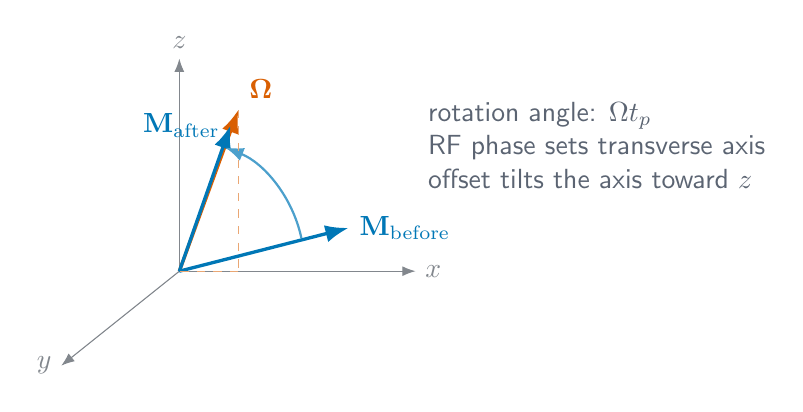
\begin{tikzpicture}[x=1cm,y=1cm,>=Latex]
  \coordinate (O) at (0,0);
  \draw[Ink!55,->] (O) -- (3.0,0) node[right] {$x$};
  \draw[Ink!55,->] (O) -- (0,2.7) node[above] {$z$};
  \draw[Ink!55,->] (O) -- (-1.5,-1.2) node[left] {$y$};
  \draw[AccentTwo,very thick,->] (O) -- (0.75,2.05) node[above right] {$\boldsymbol{\Omega}$};
  \draw[Accent,very thick,->] (O) -- (2.15,0.55) node[right] {$\mathbf{M}_{\mathrm{before}}$};
  \draw[Accent,very thick,->] (O) -- (0.65,1.85) node[left] {$\mathbf{M}_{\mathrm{after}}$};
  \draw[Accent!70,thick,->] (1.55,0.42) arc[start angle=12,end angle=68,radius=1.6];
  \node[Muted,align=left] at (5.3,1.6) {
    rotation angle: $\Omega t_p$\\
    RF phase sets transverse axis\\
    offset tilts the axis toward $z$
  };
  \draw[AccentTwo!55,dashed] (0.75,2.05) -- (0.75,0);
  \draw[AccentTwo!55,dashed] (0.75,0) -- (0,0);
\end{tikzpicture}
\end{center}

\section{Relaxation}

Free-precession intervals with relaxation use the usual exponential factors:
\[
  M_{xy}(t+\Delta t) =
    M_{xy}(t)\exp\left(-\frac{\Delta t}{T_2}\right)
    \exp(-\ii \Delta\omega\,\Delta t),
\]
\[
  M_z(t+\Delta t) =
    M_{\mathrm{th}} +
    \left(M_z(t)-M_{\mathrm{th}}\right)
    \exp\left(-\frac{\Delta t}{T_1}\right).
\]
Finite acquisition workflows assemble these intervals from pulse-sequence
parameters and then call the \code{arb10}-style kernels.

\section{Echo Conversion}

The echo utilities direct-sum a received spectrum \(S(\Delta\omega)\) over the
offset grid:
\[
  e(t) =
    \sum_k S(\Delta\omega_k)
    \exp(\ii \Delta\omega_k t)\,\Delta\omega .
\]
The implementation uses the same direct-sum convention as the MATLAB
\code{calc\_time\_domain\_echo} reference path. FID traces use the corresponding
FID conversion helper.

\section{Radiation Damping}

The deterministic radiation-damping back-action model follows the local
Measurements text convention:
\[
  T_{\mathrm{rd}} =
    \frac{2}{\gamma \mu_0 \eta M_0 Q},
\]
where \(\gamma\) is the gyromagnetic ratio, \(\eta\) is the magnetic-energy fill
factor, \(M_0\) is the equilibrium magnetization density, and \(Q\) is the
loaded probe quality factor.

The analytic on-resonance hard-pulse FID envelope used by the test suite is
\[
  |M_{xy}(t)| =
    \frac{M_0}
    {\cosh\left(t/T_{\mathrm{rd}} - \log \tan(\theta/2)\right)}.
\]
The finite-sequence implementation can add feedback during free-precession and
acquisition windows, and can optionally apply an operator-split approximation
during RF pulse matrices.

\chapter{Scalar J-Coupling Models}
\label{chap:jcoupling}

Scalar J coupling is field independent, so it can remain visible in weak or
grossly inhomogeneous magnetic fields where chemical-shift resolution is
compressed. The \code{spin\_dynamics.coupling} namespace adds a scoped set of
spin-1/2 tools for these cases. It is separate from the MATLAB-compatible Bloch
workflow layer: Bloch workflows propagate independent isochromats, while the
coupling layer propagates small dense Hilbert-space systems or evaluates
closed-form J-editing response curves.

\scopebox{Accent}{
\textbf{Use this layer for:} heteronuclear low-field J-editing curves,
known-J spectrum fitting, ideal TANGO-B filter selectivity, and exploratory
two-spin or few-spin scalar-coupled Hamiltonian simulations.
}

\scopebox{AccentTwo}{
\textbf{Current limits:} spin-1/2 only; dense matrices only; no relaxation
superoperators; no chemical exchange; no quadrupolar nuclei; no large sparse
coupled-spin networks; no full pulse-sequence compiler for arbitrary
multi-quantum pathways.
}

\section{J-Coupled Spin Cartoon}

\begin{center}
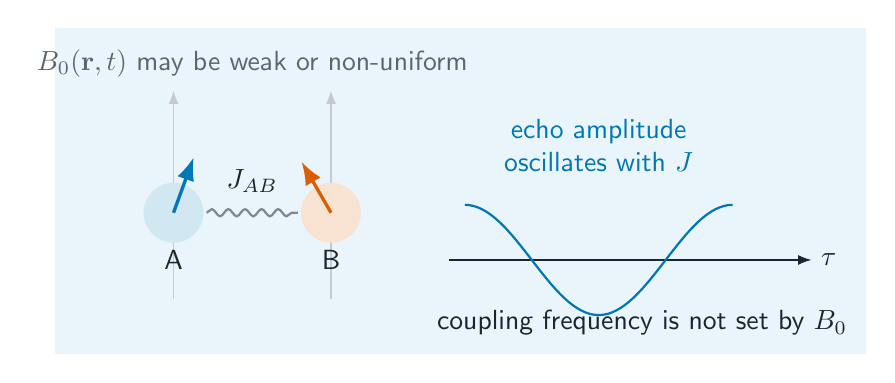
\begin{tikzpicture}[x=1cm,y=1cm,>=Latex]
  \fill[SoftBlue] (-0.5,-0.45) rectangle (9.8,3.7);
  \draw[Muted!35,->] (1.0,0.25) -- (1.0,2.9);
  \draw[Muted!35,->] (3.0,0.25) -- (3.0,2.9);
  \node[Muted] at (2.0,3.25) {$B_0(\mathbf{r},t)$ may be weak or non-uniform};
  \fill[Accent!18] (1.0,1.35) circle (0.38);
  \fill[AccentTwo!18] (3.0,1.35) circle (0.38);
  \draw[Accent,very thick,->] (1.0,1.35) -- ++(70:0.75);
  \draw[AccentTwo,very thick,->] (3.0,1.35) -- ++(120:0.75);
  \node[Ink] at (1.0,0.75) {A};
  \node[Ink] at (3.0,0.75) {B};
  \draw[Ink!55,thick,decorate,decoration={snake,amplitude=1.3pt,segment length=6pt}]
    (1.42,1.35) -- (2.58,1.35);
  \node[Ink] at (2.0,1.75) {$J_{AB}$};
  \draw[Ink,->] (4.5,0.75) -- (9.1,0.75) node[right] {$\tau$};
  \draw[Accent,thick] (4.7,1.45) cos (5.55,0.75) sin (6.4,0.05)
    cos (7.25,0.75) sin (8.1,1.45);
  \node[Accent,align=center] at (6.4,2.2) {echo amplitude\\oscillates with \(J\)};
  \node[Ink,align=left] at (6.95,-0.05) {coupling frequency is not set by \(B_0\)};
\end{tikzpicture}
\end{center}

\section{Dense Spin-1/2 Hamiltonians}

A coupled system is built from offsets \(\nu_i\) in hertz and symmetric scalar
couplings \(J_{ij}\) in hertz:

\begin{lstlisting}[language=Python]
from spin_dynamics.coupling import (
    coupled_spin_system,
    isotropic_j_hamiltonian,
    zeeman_hamiltonian,
)

system = coupled_spin_system(
    offsets_hz=[-0.35, 0.35],
    couplings_hz=[[0.0, 7.0], [7.0, 0.0]],
    labels=["A", "B"],
)
hamiltonian = zeeman_hamiltonian(system) + isotropic_j_hamiltonian(system)
\end{lstlisting}

Hamiltonian builders return angular-frequency matrices in radians per second
and use spin-1/2 operators with eigenvalues \(\pm 1/2\). The rotating-frame
offset Hamiltonian is
\[
  H_Z = 2\pi \sum_i \nu_i I_{iz}.
\]
For weakly coupled systems, the secular scalar Hamiltonian is
\[
  H_J^{\mathrm{sec}} =
    2\pi \sum_{i<j} J_{ij} I_{iz} I_{jz},
\]
while the isotropic scalar Hamiltonian is
\[
  H_J^{\mathrm{iso}} =
    2\pi \sum_{i<j} J_{ij}
      \left(I_{ix}I_{jx}+I_{iy}I_{jy}+I_{iz}I_{jz}\right).
\]
The dense propagator evaluates
\[
  \rho(t) = U(t)\rho(0)U^\dagger(t),
  \qquad
  U(t)=\exp\left(-\ii Ht\right),
\]
and is intended for small systems where dense matrices are acceptable.

\section{Inhomogeneous B0/B1 Isochromats}

The bridge between the coupled-spin layer and the Bloch workflow layer is a
coupled isochromat ensemble. Each isochromat contains the same scalar-coupled
spin network, but samples a different local field and receive weight. For
isochromat \(k\), the local spin offsets are
\[
  \nu_{i,k} = \nu_i^{(0)} + s_i\,\Delta\nu_k ,
\]
where \(\nu_i^{(0)}\) is the base spin offset, \(\Delta\nu_k\) is the local
B0 offset in hertz, and \(s_i\) is a per-spin offset scale. The default
\(s_i=1\) adds the same field offset to every spin. Heteronuclear or
carrier-specific models can supply different scales.

During an RF or spin-lock interval, the nominal nutation frequency is scaled by
the local transmit field:
\[
  \omega_{1,k} = b_{1,k}^{\mathrm{tx}} \omega_1 .
\]
The ensemble signal is accumulated as
\[
  S = \sum_k w_k b_{1,k}^{\mathrm{rx}}
      \operatorname{Tr}\!\left(\rho_k D\right),
\]
where \(w_k\) is the isochromat weight, \(b_{1,k}^{\mathrm{rx}}\) is the local
receive scale, and \(D\) is the detection operator.

\begin{lstlisting}[language=Python]
from spin_dynamics.coupling import (
    coupled_isochromat_ensemble,
    free_precession_step,
    rf_step,
    simulate_coupled_isochromat_sequence,
)

ensemble = coupled_isochromat_ensemble(
    system,
    b0_offsets_hz=[-2.0, 0.0, 2.0],
    weights=[0.25, 0.5, 0.25],
    b1_tx_scale=[0.9, 1.0, 1.1],
    b1_rx_scale=[1.0, 1.0, 0.8],
)

result = simulate_coupled_isochromat_sequence(
    ensemble,
    [
        rf_step(duration=0.25, nutation_hz=1.0, phase=1.5708),
        free_precession_step(duration=0.01),
    ],
    initial_axis="x",
    detect_axis="x",
)
\end{lstlisting}

For time-varying fields, each sequence step may override the ensemble B0
offsets or B1 transmit scale. This keeps the first implementation close to the
existing isochromat approach: the coupled-spin Hilbert space is dense and small,
while field inhomogeneity is represented by an outer ensemble sum.

\section{Low-Field J-Editing}

Analytic J-editing helpers model response curves as sums of field-independent
cosine modulations:
\[
  s(\tau) =
    b + \sum_m a_m
      \cos^{p_m}\!\left(2\pi N J_m \tau\right),
\]
where \(\tau\) is the encoding time, \(N\) is the number of encoding cycles,
\(J_m\) is a known or hypothesized coupling in hertz, \(a_m\) is its amplitude,
and \(p_m\) is an optional multiplicity exponent. Proton-detected models use
\(p_m=1\). Carbon-detected \(\mathrm{CH}_n\) groups use \(p_m=n\).

\begin{lstlisting}[language=Python]
from spin_dynamics.coupling import (
    carbon_detected_j_modulation,
    fit_known_j_spectrum,
    j_modulation_curve,
)

signal = j_modulation_curve(
    encoding_times,
    couplings_hz=[125.0, 160.0],
    amplitudes=[0.85, 0.15],
)

carbon_signal = carbon_detected_j_modulation(
    encoding_times,
    couplings_hz=[125.0, 160.0],
    abundances=[0.85, 0.15],
    proton_counts=[2, 1],
)

fit = fit_known_j_spectrum(
    encoding_times,
    signal,
    couplings_hz=[125.0, 160.0],
    include_background=False,
)
\end{lstlisting}

\code{fit\_known\_j\_spectrum} solves a linear least-squares problem once the
candidate \(J_m\) values are supplied. It returns amplitudes, optional
background, fitted signal, residual, rank, and residual norm.

\section{TANGO-B Filtering}

The ideal TANGO-B helper evaluates the coupled-spin transverse filter envelope
\[
  A(J;t_d) = \sin^2\!\left(\pi J t_d\right).
\]
When a target coupling \(J_\star\) and positive odd order \(n\) are supplied,
the delay is selected as
\[
  t_d = \frac{n}{2J_\star}.
\]

\begin{lstlisting}[language=Python]
from spin_dynamics.coupling import tango_b_filter

response = tango_b_filter(
    couplings_hz,
    target_coupling_hz=160.0,
    order=3,
)
\end{lstlisting}

This model is idealized: it reports the scalar-coupling selectivity envelope,
not RF imperfections, relaxation, diffusion, or probe filtering.

\section{SLIC Response}

Spin-lock induced crossing (SLIC) is modeled by adding an RF spin-lock
Hamiltonian to the static coupled-spin Hamiltonian:
\[
  H_{\mathrm{SLIC}} =
    H_Z + H_J^{\mathrm{iso}}
    + 2\pi \omega_1 \sum_i I_{ix}.
\]
The helper scans spin-lock nutation frequencies \(\omega_1\) in hertz and
returns the remaining transverse magnetization and its corresponding dip:

\begin{lstlisting}[language=Python]
from spin_dynamics.coupling import (
    coupled_spin_system,
    simulate_slic_spectrum,
    two_spin_slic_transfer_time,
)

system = coupled_spin_system(
    offsets_hz=[-0.35, 0.35],
    couplings_hz=[[0.0, 7.0], [7.0, 0.0]],
)
duration = two_spin_slic_transfer_time(offset_difference_hz=0.7)
result = simulate_slic_spectrum(
    system,
    nutation_frequencies_hz,
    spin_lock_time=duration,
)
\end{lstlisting}

For a nearly equivalent two-spin system, the SLIC dip is expected near the
coupling frequency. The helper is exploratory and dense; broad homonuclear
networks will need sparse or specialized methods.

\chapter{Pulsed NQR Models}
\label{chap:nqr}

Nuclear quadrupole resonance is driven by the interaction between a nuclear
quadrupole moment and the local electric-field-gradient (EFG) tensor. The
\code{spin\_dynamics.nqr} namespace adds a scoped quadrupolar extension for
solid-state pulsed NQR experiments. It is intentionally separate from the
spin-1/2 Bloch and scalar-coupling layers.

\scopebox{Accent}{
\textbf{Use this layer for:} selective pulsed NQR of one quadrupolar site,
spin-1 nitrogen-14 transition metadata, fixed-orientation single-crystal
calculations, powder averages over local EFG orientations, SLSE echo trains,
two-frequency population transfer, and exploratory weak-B0 perturbations.
}

\scopebox{AccentTwo}{
\textbf{Current limits:} dense single-site matrices only; selective RF pulses
only; phenomenological echo decay rather than full relaxation superoperators;
no simultaneous multi-frequency excitation; no full nonselective shaped-pulse
Hamiltonian propagation; no multi-site coupling between quadrupolar nuclei.
}

\section{Quadrupolar Site Model}

A quadrupolar site is described in the EFG principal-axis system. The zero-field
Hamiltonian used by the Python helper is
\[
  H_Q = \frac{2\pi \nu_Q}{3}
  \left[
    3 I_z^2 - I(I+1)\mathbf{1}
    + \eta\left(I_x^2 - I_y^2\right)
  \right],
\]
where \(I\) is the spin quantum number, \(\nu_Q\) is the quadrupole-frequency
parameter in hertz, and \(0 \le \eta \le 1\) is the EFG asymmetry parameter.
Hamiltonians are represented in radians per second.

Weak Zeeman perturbations can be added as
\[
  H_Z = -2\pi \gamma\, \mathbf{B}_0\cdot\mathbf{I},
\]
where \(\mathbf{B}_0\) is expressed in the EFG principal-axis system for the
current crystallite orientation. The default is \(B_0=0\), which is the usual
NQR case.

\begin{lstlisting}[language=Python]
from spin_dynamics.nqr import QuadrupolarSite, diagonalize_site

site = QuadrupolarSite(
    spin=1,
    isotope="14N",
    quadrupole_frequency_hz=900e3,
    eta=0.3,
)

eigensystem = diagonalize_site(site)
for transition in eigensystem.transitions:
    print(transition.label, transition.frequency_hz)
\end{lstlisting}

For spin-1 at zero field, transitions are labeled by their dominant RF
polarization in the EFG principal-axis system: \code{x}, \code{y}, and
\code{z}. For the example above the line positions are approximately
\(990\), \(810\), and \(180\) kHz.

\section{Selective Pulse Approximation}

Most practical pulsed NQR RF pulses are narrowband relative to the separation
between quadrupolar transitions. The first NQR implementation uses this
selective limit: one pulse addresses one transition and acts as an embedded
two-level rotation inside the full \((2I+1)\)-level Hilbert space.

For a transition \(|a\rangle \leftrightarrow |b\rangle\), the transition dipole
vector is
\[
  \mathbf{d}_{ab} =
  \left(
    \langle a|I_x|b\rangle,
    \langle a|I_y|b\rangle,
    \langle a|I_z|b\rangle
  \right).
\]
For a local RF direction \(\hat{\mathbf{b}}_1\), the complex drive projection
is proportional to \(\hat{\mathbf{b}}_1\cdot\mathbf{d}_{ab}\). Preserving this
signed complex projection is essential for powder averages because transmit
and receive phases must pair consistently across crystallites.

\begin{lstlisting}[language=Python]
from spin_dynamics.nqr import SelectivePulse, apply_selective_pulse

pulse = SelectivePulse(
    "x",
    duration_seconds=50e-6,
    nutation_hz=10e3,
)
\end{lstlisting}

The pulse helper also supports an optional RF frequency. If omitted, the RF is
placed on the selected transition. If supplied, the difference between the RF
frequency and transition frequency is treated as a two-level detuning.

\section{Orientations and Powder Averages}

NQR is a solid-state experiment, so the signal depends on the orientation of
the RF field relative to the local EFG principal axes. A single crystal is one
fixed orientation. A powder is represented by a normalized spherical quadrature
grid:

\begin{lstlisting}[language=Python]
from spin_dynamics.nqr import powder_average_grid, single_crystal_orientation

single = single_crystal_orientation(alpha=0.0, beta=1.57079632679)
powder = powder_average_grid(n_theta=16, n_phi=32)
\end{lstlisting}

For weak-B0 calculations, each orientation may also specify the direction of
\(B_0\) in the EFG frame. If no separate \(B_0\) direction is supplied, the
current helper uses the local RF direction as the default field direction for
that sample.

\section{SLSE Detection}

The spin-lock spin-echo (SLSE) sequence is the classic pulsed NQR detection
sequence. The initial helper models it as repeated selective pulses on a
detection transition and reports echo amplitudes at the requested echo spacing.
Echo decay is represented phenomenologically by \(T_{2e}\).

\begin{lstlisting}[language=Python]
from spin_dynamics.nqr import simulate_slse, slse_sequence

sequence = slse_sequence(
    "x",
    pulse_duration_seconds=25e-6,
    nutation_hz=10e3,
    echo_spacing_seconds=1e-3,
    num_echoes=16,
)

result = simulate_slse(
    site,
    sequence,
    orientations="powder",
    t2e_seconds=20e-3,
)
\end{lstlisting}

The returned \code{SLSEResult} includes echo times, powder-averaged echo
amplitudes, per-orientation echo amplitudes, orientation weights, transition
metadata, and the eigensystem used for the first orientation.

\section{Two-Frequency Population Transfer}

The two-frequency NQR workflow follows the perturbation-plus-detection idea
used in 2D NQR. A selective pulse on one transition changes populations in the
shared three-level spin-1 manifold; a later SLSE block detects the changed
amplitude on another transition. The normalized diagnostic is
\[
  \Delta(p,q) = \frac{S(p,q)}{S_0(q)} - 1,
\]
where \(p\) is the perturbation transition and \(q\) is the detection
transition.

\begin{lstlisting}[language=Python]
from spin_dynamics.nqr import SelectivePulse, simulate_population_transfer

transfer = simulate_population_transfer(
    site,
    SelectivePulse("x", duration_seconds=50e-6, nutation_hz=10e3),
    sequence,
    orientations="powder",
)

print(transfer.normalized_difference)
\end{lstlisting}

The diagnostic plotting example constructs a compact \(3\times3\) map over the
spin-1 \code{x}, \code{y}, and \code{z} transitions. Off-diagonal features
indicate that perturbation and detection frequencies are connected through the
same quadrupolar site.

\chapter{First Workflows}

\section{CPMG}

Application code should normally start with the public workflow runners:

\begin{lstlisting}[language=Python]
from spin_dynamics.workflows import run_tuned_cpmg

result = run_tuned_cpmg(numpts=101, maxoffs=10)
print(result.del_w.shape)
print(result.echo.shape)
print(result.snr)
\end{lstlisting}

The asymptotic CPMG runners return \code{CPMGResult} objects with the offset
grid, asymptotic magnetization, received spectrum, time-domain echo, acquisition
time vector, optional SNR, and probe label.

\section{Finite Echo Trains}

\begin{lstlisting}[language=Python]
from spin_dynamics.workflows import run_matched_cpmg_train

train = run_matched_cpmg_train(
    numpts=51,
    num_echoes=8,
    auto_refine_grid=True,
    num_workers=None,
)
\end{lstlisting}

Finite train results contain one acquired spectrum and one echo per echo index.
They also include trapezoidal echo integrals and physical echo-center times.
For long trains, use the rephasing checks or enable
\code{auto\_refine\_grid=True} so the offset grid is refined before RF matrices
are built.

\section{FID}

\begin{lstlisting}[language=Python]
from spin_dynamics.parameters import set_params_ideal_fid
from spin_dynamics.workflows.fid import sim_fid_ideal

sp, pp = set_params_ideal_fid(numpts=101)
macq, fid, tvect = sim_fid_ideal(sp, pp)
\end{lstlisting}

\section{Imaging}

\begin{lstlisting}[language=Python]
import numpy as np
from spin_dynamics.workflows import (
    make_imaging_field_maps,
    run_tuned_phase_encoded_cpmg_imaging,
    form_imaging_image,
)

rho = np.eye(8)
fields = make_imaging_field_maps(
    rho,
    b0_map=np.zeros_like(rho),
    b1_tx_map=np.ones_like(rho),
    b1_rx_map=np.ones_like(rho),
)
result = run_tuned_phase_encoded_cpmg_imaging(
    fields,
    num_echoes=4,
    ny=9,
    receive_mode="weighted",
)
image = form_imaging_image(result, mode="echo_sum")
\end{lstlisting}

Imaging workflows return raw k-space, reconstructed per-echo images, field
maps, relaxation maps, gradient metadata, and sequence timing. Image formation
is intentionally separated from acquisition so selected-echo, echo-summed,
fitted-\(\rho\), and fitted-\(T_2\) displays can be compared.

\section{Diffusion}

\begin{lstlisting}[language=Python]
from spin_dynamics.workflows import run_matched_diffusion_q_sweep

sweep = run_matched_diffusion_q_sweep(
    q_values=[20, 50],
    num_echoes=3,
    numpts=21,
    auto_refine_grid=True,
)
\end{lstlisting}

The compact matched-probe diffusion workflow is solver-validated through
\(Q=2000\). Higher-Q cases remain a stiffness target for the current NumPy
matched-probe transient solver.

\section{Time-Varying Fields}

\begin{lstlisting}[language=Python]
from spin_dynamics.workflows import (
    sinusoidal_field_waveform,
    run_ideal_time_varying_amplitude_sweep,
)

waveform = sinusoidal_field_waveform(num_echoes=16)
sweep = run_ideal_time_varying_amplitude_sweep(
    amplitudes=[0, 0.5, 1.0, 2.0],
    waveform=waveform,
    numpts=101,
    auto_refine_grid=True,
)
\end{lstlisting}

\section{WURST}

\begin{lstlisting}[language=Python]
from spin_dynamics.workflows import (
    run_ideal_wurst_inversion,
    run_matched_wurst_cpmg,
)

ideal = run_ideal_wurst_inversion(numpts=101)
matched = run_matched_wurst_cpmg(num_echoes=2, numpts=51, num_steps=64)
\end{lstlisting}

\section{Radiation Damping}

\begin{lstlisting}[language=Python]
from spin_dynamics.workflows import run_radiation_damping_fid

fid = run_radiation_damping_fid(
    probe="matched",
    fill_factor=0.7,
    equilibrium_magnetization=0.8,
    flip_angle=1.0,
    model="circuit",
    detuning=2.0e4,
)
\end{lstlisting}

Finite tuned and matched CPMG trains accept an opt-in
\code{radiation\_damping} mapping:

\begin{lstlisting}[language=Python]
from spin_dynamics.workflows import run_tuned_cpmg_train

train = run_tuned_cpmg_train(
    numpts=51,
    num_echoes=8,
    radiation_damping={
        "fill_factor": 0.7,
        "equilibrium_magnetization": 0.8,
        "model": "circuit",
        "detuning": 2.0e4,
        "apply_during_pulses": True,
    },
)
\end{lstlisting}

\section{Inverse Laplace Analysis}

\begin{lstlisting}[language=Python]
import numpy as np
from spin_dynamics.analysis import invert_t2, t2_kernel

echo_times = np.linspace(0.5e-3, 90e-3, 40)
t2_axis = np.logspace(-4, -1, 60)
signal = t2_kernel(echo_times, t2_axis) @ np.exp(-((np.log(t2_axis) + 4.5) ** 2))

result = invert_t2(
    signal,
    echo_times,
    t2_axis,
    regularization=5e-4,
    regularization_order=2,
)
\end{lstlisting}

For two-dimensional distributions, the separable forward model is
\[
  D = K_1 F K_2^{\mathsf{T}},
\]
where \(D\) is the measured data, \(F\) is the unknown distribution, and
\(K_1\), \(K_2\) are relaxation or diffusion kernels. Use
\code{invert\_t1\_t2} or \code{invert\_d\_t2} for common NMR cases.

\chapter{Examples}

The example scripts can be run from \code{PythonSpinDynamics}; each script also
works from inside \code{examples/} by adding the local source tree to
\code{sys.path} when needed.

\begin{lstlisting}[language=bash]
python examples\ideal_cpmg.py --numpts 101
python examples\ideal_fid.py --numpts 101
python examples\ideal_cpmg_train.py --numpts 101 --num-echoes 8
python examples\probe_cpmg_compare.py --numpts 101
python examples\finite_probe_train_sweeps.py --numpts 21 --num-echoes 3
python examples\matched_diffusion_cpmg.py --numpts 21 --num-echoes 3
python examples\radiation_damping_fid.py --probe matched --points 401
python examples\nmr_maser.py
python examples\heteronuclear_j_editing.py --points 33
python examples\coupled_isochromat_fields.py --points 21
\end{lstlisting}

Plotting examples require Matplotlib:

\begin{lstlisting}[language=bash]
python examples\plot_ideal_workflows.py --numpts 201 --output results\ideal_workflows.png
python examples\plot_ideal_imaging.py --pixels 6 --ny 7 --output results\ideal_imaging.png
python examples\plot_inverse_laplace.py --output results\inverse_laplace.png
python examples\plot_radiation_damping.py --output results\radiation_damping.png
python examples\plot_wurst_flow.py --numpts 41 --num-steps 64 --output results\wurst_flow.png
python examples\plot_j_editing_spectrum.py --output results\j_editing_spectrum.png
python examples\plot_j_editing_field_spread.py --output results\j_editing_field_spread.png
python examples\plot_tango_filter.py --target 160 --output results\tango_filter.png
python examples\plot_slic_two_spin.py --j-hz 7 --delta-hz 0.7 --output results\slic_two_spin.png
python examples\plot_nqr_powder_nutation.py --output results\nqr_powder_nutation.png
python examples\plot_nqr_population_transfer.py --output results\nqr_population_transfer.png
\end{lstlisting}

\chapter{Validation}

Validation fixtures live in \code{validation/fixtures}. The tests compare the
Python implementation against compact MATLAB or Octave arrays for core
rotations, echo conversion, FID, the \code{arb10} kernel, finite acquisition,
probe response, imaging, pulse-shape helpers, optimization result handling, and
public workflow result shapes.

Regenerate dependency-light fixtures with Octave or MATLAB from the
\code{PythonSpinDynamics} directory:

\begin{lstlisting}[language=bash]
matlab -batch "run('validation/octave/generate_basic_fixtures.m')"
matlab -batch "run('validation/octave/generate_imaging_fixtures.m')"
matlab -batch "run('validation/octave/generate_optimization_fixtures.m')"
matlab -batch "run('validation/octave/generate_pulse_fixtures.m')"
\end{lstlisting}

Matched-probe fixtures require MATLAB toolboxes used by the reference
implementation. Octave fixture generation skips matched-probe files when
\code{fmincon} is unavailable.

\chapter{API Reference}

This chapter documents the intended public surface. Lower-level module imports
remain available for validation and porting. For application code, start with:

\begin{lstlisting}
spin_dynamics.workflows
spin_dynamics.parameters
spin_dynamics.analysis
spin_dynamics.coupling
spin_dynamics.nqr
\end{lstlisting}

Drop into lower-level modules only when a building block is needed directly.
Use \code{spin\_dynamics.coupling} for the scoped dense scalar-coupled
spin-1/2 tools described in Chapter~\ref{chap:jcoupling}. Use
\code{spin\_dynamics.nqr} for the selective pulsed NQR tools described in
Chapter~\ref{chap:nqr}.

\section{Workflow Results}

\begin{longtable}{p{0.43\linewidth}p{0.49\linewidth}}
\toprule
Class & Purpose \\
\midrule
\code{CPMGResult} & Asymptotic CPMG spectrum, echo, time vector, SNR, and probe label. \\
\code{CPMGTrainResult} & Finite echo-train spectra, echoes, echo integrals, and sequence timing. \\
\code{CPMGIRTrainResult} & Inversion-recovery finite trains over a \code{tauvect}. \\
\code{CPMGParameterSweepResult} & Asymptotic Q or mistuning sweeps. \\
\code{CPMGFiniteParameterSweepResult} & Finite-train Q or mistuning sweeps. \\
\code{ZMagnetizationSweepResult} & Matched-probe z-magnetization Q sweeps. \\
\code{IdealTimeVaryingCPMGResult} & Final echo for ideal time-varying-field CPMG. \\
\code{ProbeTimeVaryingCPMGResult} & Probe-aware time-varying-field CPMG result. \\
\code{IdealCPMGImagingResult} & Ideal phase-encoded CPMG imaging result. \\
\code{ProbeCPMGImagingResult} & Tuned or matched phase-encoded CPMG imaging result. \\
\code{MatchedDiffusionCPMGResult} & Matched diffusion-aware CPMG train. \\
\code{MatchedDiffusionQSweepResult} & Matched diffusion Q sweep. \\
\code{WURSTInversionResult} & WURST inversion profile and pulse metadata. \\
\code{MatchedWURSTCPMGResult} & Matched WURST-CPMG echoes and spectra. \\
\code{RadiationDampingFIDResult} & Radiation-damping FID simulation and analytic comparison fields. \\
\code{SLSEResult} & NQR SLSE echo train, local orientation signals, and transition metadata. \\
\code{PopulationTransferResult} & NQR perturbation-plus-SLSE signal, reference signal, and normalized difference. \\
\bottomrule
\end{longtable}

\section{High-Level Workflows}

\begin{lstlisting}
from spin_dynamics.workflows import (
    run_ideal_cpmg, run_tuned_cpmg, run_untuned_cpmg, run_matched_cpmg,
    run_ideal_cpmg_train, run_tuned_cpmg_train,
    run_untuned_cpmg_train, run_matched_cpmg_train,
    run_ideal_cpmg_ir_train, run_tuned_cpmg_ir_train,
    run_untuned_cpmg_ir_train, run_matched_cpmg_ir_train,
    run_tuned_q_sweep, run_matched_q_sweep,
    run_tuned_mistuning_sweep, run_matched_mistuning_sweep,
    run_tuned_finite_q_sweep, run_untuned_finite_q_sweep,
    run_matched_finite_q_sweep,
    run_tuned_finite_mistuning_sweep,
    run_untuned_finite_mistuning_sweep,
    run_matched_finite_mistuning_sweep,
    run_matched_z_magnetization_q_sweep,
    run_matched_diffusion_cpmg, run_matched_diffusion_q_sweep,
    run_ideal_time_varying_cpmg_final,
    run_tuned_time_varying_cpmg_final,
    run_untuned_time_varying_cpmg_final,
    run_matched_time_varying_cpmg_final,
    run_ideal_time_varying_amplitude_sweep,
    run_tuned_time_varying_amplitude_sweep,
    run_untuned_time_varying_amplitude_sweep,
    run_matched_time_varying_amplitude_sweep,
    sinusoidal_field_waveform,
    run_ideal_wurst_inversion,
    run_matched_wurst_inversion,
    run_matched_wurst_cpmg,
    run_radiation_damping_fid,
)
\end{lstlisting}

The main CPMG runners share \code{numpts} and \code{maxoffs}. Finite train
runners add \code{num\_echoes}, relaxation constants, rephasing controls,
optional \code{auto\_refine\_grid}, and optional worker controls. Probe-aware
train runners also accept \code{q\_value} and \code{mistuning\_offset} where the
underlying probe model supports them.

\section{Imaging API}

\begin{lstlisting}
from spin_dynamics.workflows import (
    ImagingFieldMaps,
    make_imaging_field_maps,
    load_imaging_field_maps_npz,
    run_ideal_phase_encoded_cpmg_imaging,
    run_tuned_phase_encoded_cpmg_imaging,
    run_matched_phase_encoded_cpmg_imaging,
    run_t1_encoded_phase_encoded_cpmg_imaging,
    reconstruct_image_from_kspace,
    form_imaging_image,
    fit_imaging_echo_decay,
    summarize_imaging_noise_trials,
)
\end{lstlisting}

Prefer the \code{phase\_encoded} names for new code. The shorter compatibility
aliases remain available:

\begin{lstlisting}
run_ideal_cpmg_imaging
run_tuned_cpmg_imaging
run_matched_cpmg_imaging
\end{lstlisting}

\section{Parameter Constructors}

\begin{lstlisting}
from spin_dynamics.parameters import (
    set_params_ideal,
    set_params_ideal_fid,
    set_params_tuned_orig,
    set_params_untuned_orig,
    set_params_matched_orig,
    set_params_tuned_spa,
    set_params_untuned_spa,
    set_params_matched_spa,
    set_params_tuned_jmr,
    set_params_untuned_jmr,
    set_params_matched_jmr,
)
\end{lstlisting}

These constructors return dataclass instances mirroring MATLAB \code{sp},
\code{pp}, and \code{params} structures. They accept optional \code{numpts}
arguments for lightweight tests and examples while preserving MATLAB defaults
when omitted.

\section{Analysis API}

\begin{lstlisting}
from spin_dynamics.analysis import (
    t2_kernel, t1_kernel, diffusion_kernel, laplace_kernel,
    invert_laplace_1d, invert_laplace_2d,
    invert_t2, invert_t1, invert_t1_t2, invert_d_t2,
    default_regularization_strengths,
    estimate_noise_rms_from_snr,
    expected_residual_norm_from_snr,
    select_regularization_1d,
    select_regularization_2d,
)
\end{lstlisting}

For one-dimensional relaxation distributions, use:

\begin{lstlisting}
invert_t2
invert_t1
\end{lstlisting}

For separable two-dimensional maps, use:

\begin{lstlisting}
invert_t1_t2
invert_d_t2
\end{lstlisting}

The \code{select\_regularization\_*} helpers choose Tikhonov strengths from an
RMS SNR estimate.

\section{Core Numerical API}

\begin{lstlisting}
from spin_dynamics.core.echo import (
    calc_time_domain_echo,
    calc_time_domain_echo_arb,
    calc_fid_time_domain,
)
from spin_dynamics.core.rotations import (
    calc_rotation_matrix,
    calc_rot_axis_arba3,
    calc_rot_axis_arba4,
    calc_v0crit,
    sim_spin_dynamics_asymp_mag3,
    sim_spin_dynamics_exc,
)
from spin_dynamics.core.kernels import (
    sim_spin_dynamics_arb7,
    sim_spin_dynamics_arb10,
    sim_spin_dynamics_arb10_chunked,
    sim_spin_dynamics_arb10_diffusion,
    sim_spin_dynamics_arb10_radiation_damping,
)
from spin_dynamics.core.isochromats import (
    analyze_rephasing,
    check_rephasing,
    estimate_rephase_time,
    recommended_numpts_for_rephasing,
)
\end{lstlisting}

Core functions are intended for validation, debugging, and continued porting.
They are closer to MATLAB's array contracts than the workflow layer.

\section{Probe and Pulse API}

\begin{lstlisting}
from spin_dynamics.probes.tuned import (
    tuned_probe_lp,
    tuned_probe_rx,
    tuned_probe_rx_tf,
    calc_rot_axis_tuned_probe_lp_orig2,
    calc_masy_tuned_probe_lp_orig,
)
from spin_dynamics.probes.untuned import (
    untuned_probe_lp,
    untuned_probe_rx,
    untuned_probe_rx_tf,
    calc_rot_axis_untuned_probe_lp,
    calc_masy_untuned_probe_lp,
)
from spin_dynamics.probes.matched import (
    matching_network_design2,
    find_coil_current,
    find_coil_current_wurst,
    matched_probe_rx,
    calc_rot_axis_matched_probe,
    calc_masy_matched_probe_orig,
    calc_masy_matched_nut,
)
from spin_dynamics.pulses import (
    quantize_phase,
    create_wurst_pulse,
    adjust_untuned_segment_lengths,
    tuned_rectangular_pulse_response,
    untuned_rectangular_pulse_response,
    matched_rectangular_pulse_response,
    matched_wurst_pulse_response,
)
\end{lstlisting}

\section{Noise, Motion, and Radiation Damping}

\begin{lstlisting}
from spin_dynamics.noise import (
    NoiseSpec,
    add_received_noise,
    estimate_matched_filter_snr,
    ideal_noise_density,
    tuned_probe_output_noise_density,
    untuned_probe_output_noise_density,
    matched_probe_output_noise_density,
)
from spin_dynamics.motion import (
    make_motion_field_maps_2d,
    initialize_ensemble_from_density,
    advect_diffuse_positions,
    move_ensemble,
    apply_free_precession,
    apply_rf_rotation,
    free_precession_with_motion_step,
    receive_signal,
    transverse_b1_magnitude,
)
from spin_dynamics.radiation_damping import (
    radiation_damping_time,
    proton_thermal_magnetization_density,
    water_proton_sample,
    hyperpolarized_proton_sample,
    normalized_radiation_damping_weights,
    radiation_damping_probe_from_tuned,
    radiation_damping_probe_from_matched,
    initial_state_from_flip_angle,
    analytic_radiation_damping_envelope,
    simulate_radiation_damping,
    simulate_radiation_damping_fid,
    simulate_nmr_maser,
)
\end{lstlisting}

\section{Scalar Coupling API}

\begin{lstlisting}
from spin_dynamics.coupling import (
    CoupledSpinSystem,
    CoupledIsochromatEnsemble,
    CoupledIsochromatStep,
    CoupledIsochromatSequenceResult,
    coupled_spin_system,
    coupled_isochromat_ensemble,
    free_precession_step,
    rf_step,
    simulate_coupled_isochromat_sequence,
    spin_operator,
    total_operator,
    product_operator,
    zeeman_hamiltonian,
    secular_j_hamiltonian,
    isotropic_j_hamiltonian,
    rf_hamiltonian,
    equilibrium_density,
    evolve_density,
    expectation,
    j_modulation_curve,
    proton_detected_j_modulation,
    carbon_detected_j_modulation,
    tango_b_filter,
    fit_known_j_spectrum,
    JEditingFitResult,
    simulate_slic_spectrum,
    two_spin_slic_transfer_time,
    SLICSpectrumResult,
)
\end{lstlisting}

\begin{longtable}{p{0.42\linewidth}p{0.50\linewidth}}
\toprule
Object & Purpose \\
\midrule
\code{CoupledSpinSystem} & Validated small spin-1/2 system with offsets and scalar couplings in hertz. \\
\code{CoupledIsochromatEnsemble} & Ensemble of local B0/B1 field samples for one coupled-spin system. \\
\code{free\_precession\_step}, \code{rf\_step} & Sequence-step builders with optional time-varying B0/B1 overrides. \\
\code{simulate\_coupled\_isochromat\_sequence} & Dense coupled-spin sequence propagation over an isochromat ensemble. \\
\code{spin\_operator}, \code{total\_operator}, \code{product\_operator} & Dense spin-1/2 operator builders. \\
\code{zeeman\_hamiltonian} & Rotating-frame offset Hamiltonian in radians per second. \\
\code{secular\_j\_hamiltonian} & Weak-coupling \(I_zI_z\) scalar Hamiltonian. \\
\code{isotropic\_j\_hamiltonian} & Isotropic scalar Hamiltonian for strongly coupled spin-1/2 systems. \\
\code{rf\_hamiltonian} & RF nutation Hamiltonian for selected spins. \\
\code{equilibrium\_density}, \code{evolve\_density}, \code{expectation} & Minimal dense density-matrix utilities. \\
\code{j\_modulation\_curve} & Sum of cosine J-modulation components. \\
\code{proton\_detected\_j\_modulation} & Proton-detected low-field J-editing response. \\
\code{carbon\_detected\_j\_modulation} & Carbon-detected \(\cos^n\) J-editing response for \(\mathrm{CH}_n\) groups. \\
\code{tango\_b\_filter} & Ideal TANGO-B scalar-coupling filter envelope. \\
\code{fit\_known\_j\_spectrum} & Least-squares amplitudes for supplied J-coupling positions. \\
\code{simulate\_slic\_spectrum} & Spin-lock response scan for dense coupled-spin systems. \\
\bottomrule
\end{longtable}

\section{NQR API}

\begin{lstlisting}
from spin_dynamics.nqr import (
    QuadrupolarSite,
    NQRTransition,
    NQREigensystem,
    spin_matrices,
    quadrupole_hamiltonian,
    zeeman_hamiltonian,
    nqr_hamiltonian,
    diagonalize_site,
    OrientationSample,
    single_crystal_orientation,
    powder_average_grid,
    SelectivePulse,
    apply_selective_pulse,
    transition_drive_scale,
    slse_sequence,
    simulate_slse,
    simulate_population_transfer,
    SLSEResult,
    PopulationTransferResult,
)
\end{lstlisting}

\begin{longtable}{p{0.42\linewidth}p{0.50\linewidth}}
\toprule
Object & Purpose \\
\midrule
\code{QuadrupolarSite} & One quadrupolar nucleus in the EFG principal-axis system. \\
\code{spin\_matrices} & Dense angular-momentum operators for arbitrary integer or half-integer spin. \\
\code{quadrupole\_hamiltonian} & Zero-field quadrupole Hamiltonian in radians per second. \\
\code{zeeman\_hamiltonian} & Optional weak-B0 perturbation in radians per second. \\
\code{diagonalize\_site} & Energy levels, transition frequencies, and transition dipole vectors. \\
\code{OrientationSample} & One EFG orientation relative to lab RF and optional B0 fields. \\
\code{single\_crystal\_orientation} & One fixed orientation sample. \\
\code{powder\_average\_grid} & Normalized spherical powder quadrature grid. \\
\code{SelectivePulse} & Rectangular selective pulse on one transition. \\
\code{apply\_selective\_pulse} & Embedded two-level RF propagation in the energy basis. \\
\code{slse\_sequence} & Convenience builder for SLSE detection. \\
\code{simulate\_slse} & Selective-pulse SLSE echo train for a fixed orientation or powder. \\
\code{simulate\_population\_transfer} & Perturbation pulse plus SLSE detection for 2D NQR diagnostics. \\
\bottomrule
\end{longtable}

\section{Optimization API}

\begin{lstlisting}
from spin_dynamics.optimization import (
    spa_pulse_list,
    rectangular_refocusing_lengths,
    evaluate_tuned_refocusing_pulse,
    evaluate_untuned_refocusing_pulse,
    evaluate_matched_refocusing_pulse,
    evaluate_ideal_v0crit_refocusing_pulse,
    evaluate_ideal_v0crit_excited_refocusing_pulse,
    evaluate_ideal_time_varying_refocusing_pulse,
    optimize_tuned_refocusing_phases,
    optimize_untuned_refocusing_phases,
    optimize_matched_refocusing_phases,
    optimize_ideal_v0crit_refocusing_phases,
    optimize_ideal_v0crit_excited_refocusing_phases,
    optimize_ideal_time_varying_refocusing_phases,
    run_tuned_refocusing_multistart,
    run_untuned_refocusing_multistart,
    run_matched_refocusing_multistart,
    run_ideal_v0crit_refocusing_multistart,
    run_ideal_v0crit_excited_refocusing_multistart,
    run_ideal_time_varying_refocusing_multistart,
    evaluate_tuned_excitation_pulse,
    evaluate_tuned_inverse_excitation_pulse,
    optimize_tuned_excitation_phases,
    optimize_tuned_inverse_excitation_phases,
    run_tuned_excitation_multistart,
    run_tuned_inverse_excitation_multistart,
    run_tuned_excitation_inverse_pipeline,
    multistart_to_matlab_results,
    save_multistart_results_npz,
    load_optimization_results,
    summarize_matlab_results,
    select_matlab_result_program,
    analyze_matlab_optimization_results,
    analyze_tuned_inverse_result_pair,
)
\end{lstlisting}

The optimization layer is useful for compact pulse-design studies and
MATLAB-style result inspection. Broad historical \code{fmincon} parity and
strong inverse-excitation cancellation parity remain validation targets.

\chapter{Known Gaps}

The Python port is intentionally conservative where MATLAB parity still
matters. The largest remaining gaps are broader high-Q matched-probe validation,
full historical MATLAB \code{.mat} structure parity, broad \code{fmincon}
parity, paper-level scalar-coupling fixture comparisons, relaxation-aware
coupled-spin pulse-sequence runners, full nonselective quadrupolar pulse
propagation, experimental NQR fixture comparisons, and acceleration backends
beyond the current NumPy implementation.

New work should add small reference fixtures first, then a NumPy implementation,
then optional acceleration or plotting once numerical behavior is pinned down.

\end{document}
